\documentclass[aspectratio=169]{beamer}

%https://en.wikibooks.org/wiki/LaTeX/Presentations
%\AtBeginSection[]{\subsection{}}
%\beamertemplatenavigationsymbolsempty

\usetheme{Singapore}
%\usetheme{Rochester}
%\usetheme{JD}
%\usetheme{PaloAlto}
%\usetheme{Copenhagen}
%\usecolortheme{orchid}
%\usecolortheme{whale}

%\usecolortheme{Antibes}
\useoutertheme[hideothersubsections]{sidebar}
%\usetheme{Rochester}
\usecolortheme{orchid}
\useoutertheme[hideothersubsections]{sidebar}
\setbeamertemplate{itemize items}[circle]
\setbeamertemplate{section in toc}[circle]

\setbeamertemplate{frametitle}{\vspace{-1cm}{\usebeamercolor[fg]{structure}\bfseries\insertframetitle}}


\usepackage{helvet}

\usepackage{listings}

\usepackage{hyperref}


\title
    [Main Project]
    {\textbf{Multi-core RISC Processor Design \& Implementation}}
\subtitle{Demonstration Viva}

\author
    [B. Lancaster]
    {Ben Lancaster}
\institute
    [\hypersetup{urlcolor=jdgrey}%
     \href{https://bendl.me/}{https://bendl.me}
    ]
    {201280376\\
    ELEC5881M - Main Project}
\date
    [12/2016]
    {\today}



\begin{document}

\begin{frame}[plain]
\titlepage
\end{frame}

\begin{frame}{Quick Links}
\begin{itemize}
    \item GitHub repository: \url{https://github.com/bendl/vmicro16}
    \item Full Report: \url{https://github.com/bendl/vmicro16/blob/master/docs/reports/build/ELEC5881M_Ben_Lancaster_201280376_Final.pdf}
\end{itemize}
\end{frame}

\begin{frame}
\vspace{-1cm}
\begin{columns}[t]
        \begin{column}{.5\textwidth}
            \tableofcontents[sections={1-3}]
        \end{column}
        \begin{column}{.5\textwidth}
            \tableofcontents[sections={4-5}]
        \end{column}
    \end{columns}
\end{frame}

\section{Introduction}
\frame{\tableofcontents[currentsection, subsectionstyle=show/show/hide]}

\subsection{Why Multi-core?}
\begin{frame}{Why Multi-core?}
\begin{alertblock}{Block Title}
Lorem ipsum dolor sit amet, consectetur adipisicing elit, 
sed do eiusmod tempor incididunt ut labore et 
dolore magna aliqua.
\end{alertblock}
\end{frame}

\subsection{Why RISC?}
\begin{frame}{Why RISC?}
\end{frame}

\section{Top Level Design}
\frame{\tableofcontents[currentsection, subsectionstyle=show/show/hide]}

\subsection{Overview}
\begin{frame}{Overview}
\textbf{What this project produces:}
\begin{itemize}[<+->]\setlength\itemsep{1em}
    \item{\textbf{System-on-Chip with multi-processor functionality}\\
    Tested on FPGA hardware with 1-96 CPU cores.}
    \item{\textbf{Custom 16-bit RISC CPU}\\
    With interrupts and its own Instruction Set Architecture (ISA).}
    \item{\textbf{Aimed at Design Engineers, not end users}\\
    Project is provided as source code/design files for Design Engineers to customise and implement in hardware themselves.}
    \item{\textbf{Software/Assembly compiler}\\
    PRCO304 programming language/Intel assembly syntax.}
\end{itemize}
\end{frame}

\begin{frame}{Top Level Hierarchy}
\vspace{-.3cm}
\begin{figure}
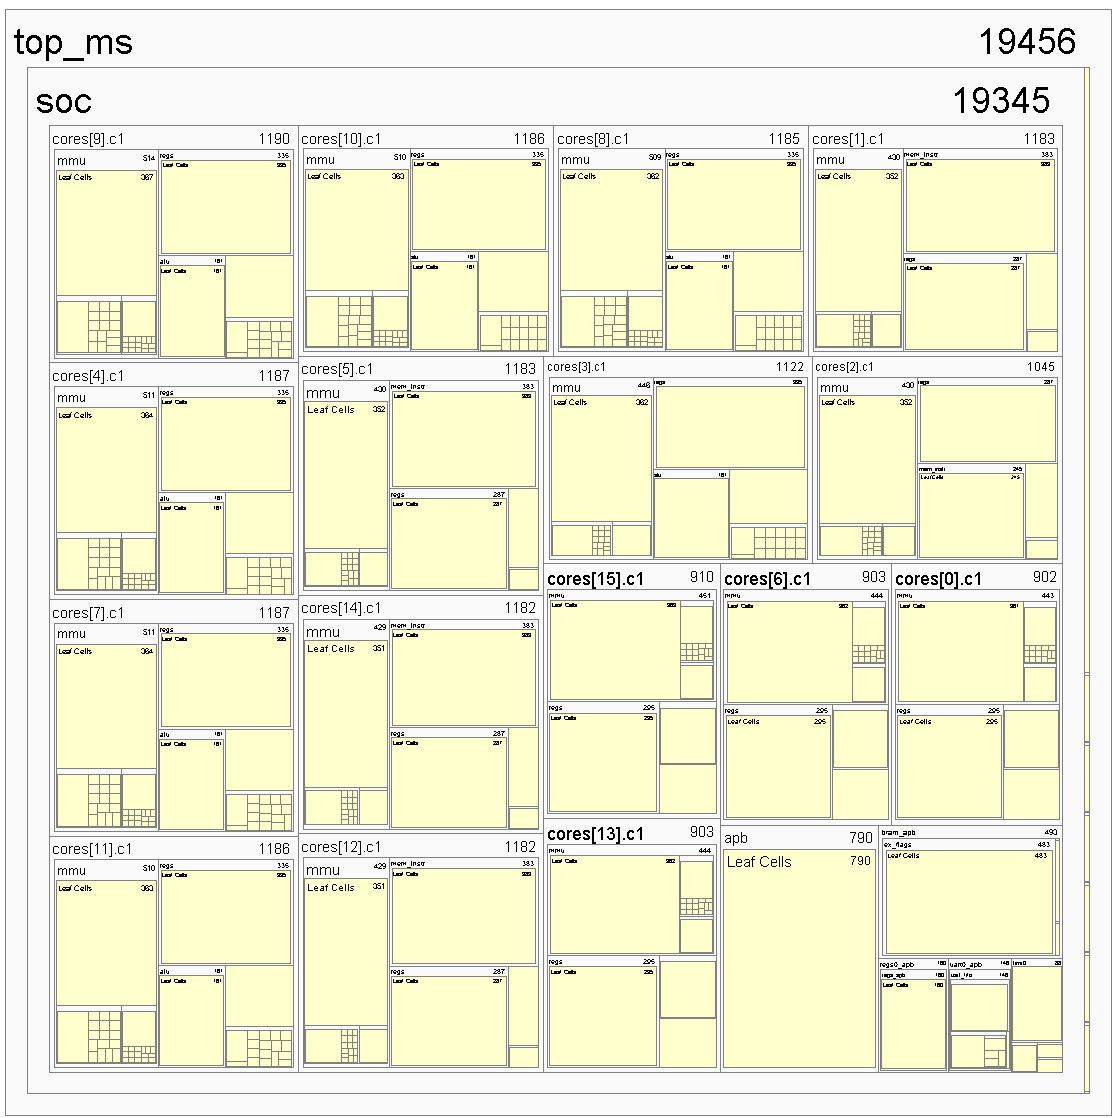
\includegraphics[width=7.5cm]{soc_layout_schem}
\end{figure}
\end{frame}

\subsection{Memory Map}
\begin{frame}{Memory Map}
\begin{columns}
\column{0.5\textwidth}
\begin{figure}
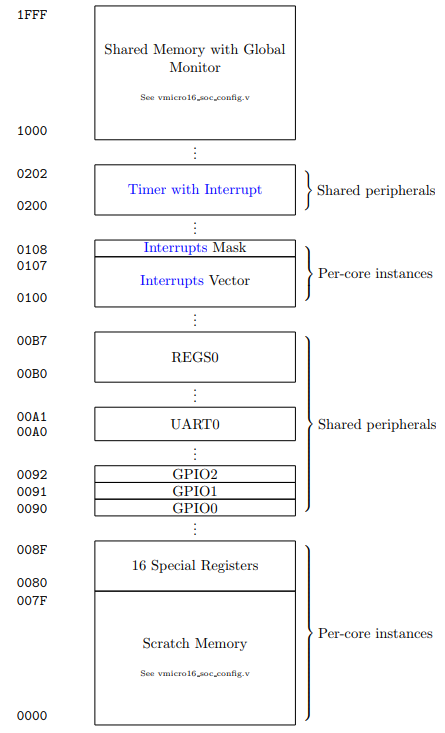
\includegraphics[width=4cm]{memory_map}
\end{figure}
\column{0.5\textwidth}
\begin{itemize}
    \item \textbf{Shared Memory with Global Monitor}
    \item Timer with Interrupt
    \item Per-core Interrupt Vector and Mask
    \item Shared Register Set
    \item UART Transceiver
    \item Multiple GPIO ports
    \item Per-core scratch memory
    \item \textbf{Per-core Special Registers}
    \item Customisable by designers
\end{itemize}
\end{columns}
\end{frame}

\subsection{Interconnect}
\begin{frame}{Interconnect}

\end{frame}

\subsection{Interrupts}
\begin{frame}[t]{Interrupts}
\begin{columns}[t]
\column{0.5\textwidth}
\begin{figure}
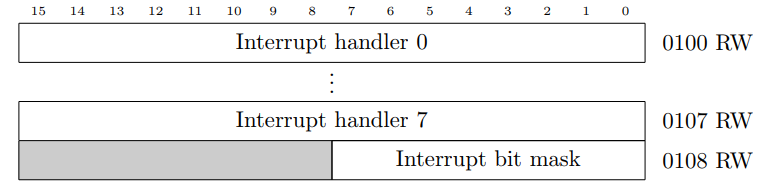
\includegraphics[width=\textwidth]{rinterrupts}\\
\vspace{.5cm}
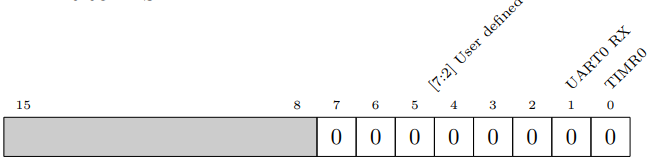
\includegraphics[width=\textwidth]{rinterruptsmask}
\end{figure}
\column{0.5\textwidth}
\begin{figure}
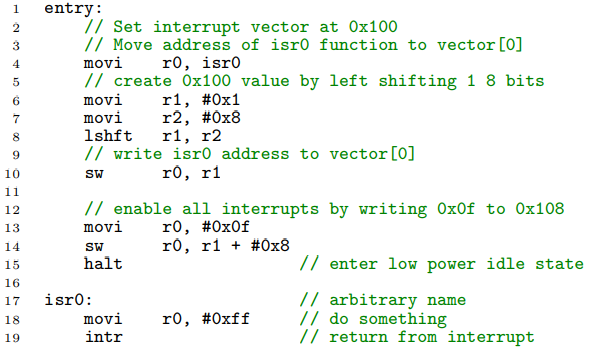
\includegraphics[width=\textwidth]{vinterrupts}
\end{figure}
\end{columns}
\vspace{1cm}
Demo: 2 Core LED toggle (GPIO0) with TIMR0 1s interrupt (interrupts\_2.s)
\end{frame}

\begin{frame}{Timer Interrupt Example}
    \begin{figure}
        \centering
        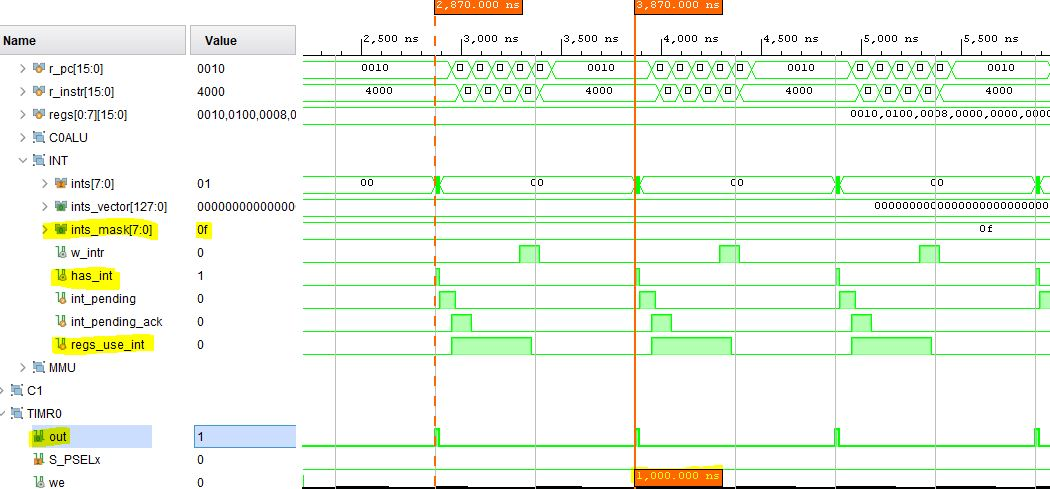
\includegraphics[width=0.9\textwidth]{interrupts}
        \caption{TIMR0 1us interrupt with context switching}
        \label{fig:my_label}
    \end{figure}
\end{frame}

\begin{frame}{Timer Peripheral Registers}
    \begin{figure}
        \centering
        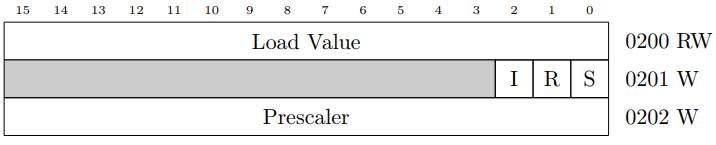
\includegraphics[width=0.9\textwidth]{rtimer}
        \caption{$t = 20{ns} * {load} * {prescaler}$}
        \label{fig:my_label}
    \end{figure}
    Resolution (32-bit timer): 20ns to 85s.
    
    Examples: 
    \begin{itemize}
        \item For 1us: Load = 0x32, Prescaler = 0 (20ns * 0x32 = 1000ns)
        \item For 1s:  Load = 0x1000, Prescaler = 0x3000 (demo)\\(20ns * 0x1000 * 0x3000 = approx. 1s)
    \end{itemize}
\end{frame}

\section{Multi-core Functionality}
\frame{\tableofcontents[currentsection, subsectionstyle=show/show/hide]}
\subsection{HW/SW Requirements}
\begin{frame}{HW/SW Requirements}
\begin{columns}[t]
\column{0.5\textwidth}
Hardware:
\begin{itemize}[<+->]
    \item \textbf{Bus Arbitration}\\ (scheduling: priority, rotating, etc.)
    \item \textbf{Atomic functions}\\ (atomic versions of load/store to prevent race conditions)
    \item Per-core instruction memory
    \item Per-core context-switching for interrupt handling
\end{itemize}
\column{0.5\textwidth}
Software:
\begin{itemize}[<+->]
    \item Semaphores/Mutexes\\ (exclusive memory access)
    \item Thread synchronisation\\ (memory barriers)
    \item \textbf{Context identification}\\ What core am I?\\ How many cores?\\ How much memory?
\end{itemize}
\end{columns}
\end{frame}

\subsection{Context Identification}
\begin{frame}[fragile]{Context Identification}
\begin{columns}
\column{0.5\textwidth}
\begin{figure}
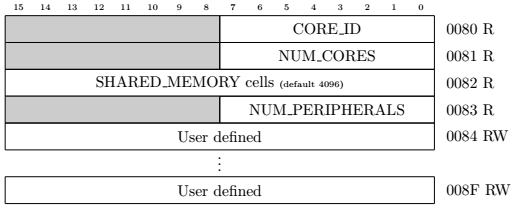
\includegraphics[width=\textwidth]{sregs}
\caption{Special Registers 0x0080 to 0x008F}
\end{figure}
\column{0.5\textwidth}
\begin{lstlisting}[basicstyle=\scriptsize]
entry:
    // get core idx 0x80 in r7
    movi    r7, #0x80
    lw      r7, r7

    // Branch away if not core 0
    cmp     r7, r0
    movi    r0, exit
    br      r0, BR_NE 
    
    // Core 0 only instructions
    nop     r0, r0
    nop     r0, r0
    nop     r0, r0
    
exit:
    halt    r0, r0    
\end{lstlisting}
\end{columns}
\end{frame}

\section{Results}
\frame{\tableofcontents[currentsection, subsectionstyle=show/show/hide]}
\begin{frame}{Results}
\end{frame}
\subsection{Results 1}
\begin{frame}{Results 1}
\end{frame}

\section{Conclusion}
\frame{\tableofcontents[currentsection, subsectionstyle=show/show/hide]}

\subsection{Accomplishments}
\begin{frame}{Accomplishments}
\begin{itemize}
    \item \textbf{Near complete System-on-Chip design with various peripherals}\\
    Timers, GPIO, UART, Registers, Memory
    
    \item \textbf{Common multi-thread/core synchronisation primitives}\\
    Semaphores, Mutexes, Memory Barriers, Atomic Instructions
    
    \item \textbf{AMBA APB bus interface with Global Monitor}\\
    Timers, GPIO, UART, Registers, Memory
    
    \item \textbf{Working shared bus arbitration}\\
    Schedules access to shared resources
    
    \item \textbf{Working FPGA implementation for a 96 core design}\\
    Nearly fills Cyclone V FPGA on the DE1-SoC
    
    \item \textbf{Interrupts with hardware context-switching}\\
    Low latency to react to interrupt
    
    \item \textbf{Acknowledges design limitations and attempts to overcome}\\
    LUT resources, block memories, power and temperature requirements
\end{itemize}
\end{frame}

\subsection{Future Improvements}
\begin{frame}{Future Improvements}

\begin{itemize}
    \item \textbf{Working Global Reset}\\
    Timers, GPIO, UART, Registers, Memory
    
    \item \textbf{Common multi-thread/core synchronisation primitives}\\
    Semaphores, Mutexes, Memory Barriers, Atomic Instructions
    
    \item \textbf{AMBA APB bus interface with Global Monitor}\\
    Timers, GPIO, UART, Registers, Memory
    
    \item \textbf{Working shared bus arbitration}\\
    Schedules access to shared resources
    
    \item \textbf{Working FPGA implementation for a 96 core design}\\
    Nearly fills Cyclone V FPGA on the DE1-SoC
    
    \item \textbf{Interrupts with hardware context-switching}\\
    Low latency to react to interrupt
    
    \item \textbf{Acknowledges design limitations and attempts to overcome}\\
    LUT resources, block memories, power and temperature requirements
\end{itemize}
\end{frame}

\end{document}
